\documentclass[8pt,a4paper,compress]{beamer}

\usepackage{/home/siyer/lib/slides}

\title{Analysis of Algorithms}
\date{}

\begin{document}
\begin{frame}
\vfill
\titlepage
\end{frame}

\begin{frame}
\frametitle{Outline}
\tableofcontents
\end{frame}

\section{Complexity of Algorithms}
\begin{frame}[fragile]
\pause

Questions that arise when we write programs that process large amounts of data
\begin{itemize}
\item How long will my program take, ie, what's the time complexity of my program?
\item How much memory will my program need, ie, what's the space complexity of my program?
\end{itemize}
\end{frame}

\section{Time Complexity}
\begin{frame}[fragile]
\pause

Example (3-sum problem)
\begin{lstlisting}[language=Java]
package edu.princeton.cs.algs4;

public class ThreeSum {
    public static int count(int[] a) {
        int N = a.length;
        int cnt = 0;
        for (int i = 0; i < N; i++) {
            for (int j = i + 1; j < N; j++) {
                for (int k = j + 1; k < N; k++) {
                    if (a[i] + a[j] + a[k] == 0) { 
                        cnt++; 
                    }
                }
            }
        }
        return cnt;
    }
    
    public static void main(String[] args)  { 
        In in = new In(args[0]);
        int[] a = in.readAllInts();
        Stopwatch timer = new Stopwatch();
        int cnt = count(a);
        StdOut.println("elapsed time = " + timer.elapsedTime());
        StdOut.println(cnt);
    } 
}
\end{lstlisting}

\pause

\begin{lstlisting}[language={}]
$ java edu.princeton.cs.algs4.ThreeSum 1Kints.txt 
elapsed time = 0.334
70
$ java edu.princeton.cs.algs4.ThreeSum 2Kints.txt 
elapsed time = 2.643
528
\end{lstlisting}
\end{frame}

\begin{frame}[fragile]
\pause

We can carry out experimental analysis of the order of growth (aka running time) $T(N)$ of a program using a stopwatch, where $N$ is the input size

\pause
\bigskip

\lstinline{Stopwatch} API
\begin{center}
\begin{tabular}{cc}
method & description \\ \hline
\lstinline$Stopwatch()$ & create a stopwatch \\
\lstinline$double elapsedTime()$ & elapsed time since creation
\end{tabular} 
\end{center}

\pause
\bigskip

\lstinline{Stopwatch} implementation
\begin{lstlisting}[language=Java]
package edu.princeton.cs.algs4;

public class Stopwatch {
    private final long start;
    
    public Stopwatch() { 
        start = System.currentTimeMillis(); 
    }
    
    public double elapsedTime() {
        return (System.currentTimeMillis() - start) / 1000.0;
    }
}
\end{lstlisting}
\end{frame}

\begin{frame}[fragile]
\pause

A \lstinline{Stopwatch} client that produces experimental data for \lstinline{ThreeSum}
\begin{lstlisting}[language=Java]
package edu.princeton.cs.algs4;

public class DoublingTest {
    public static double timeTrial(int N) {
        int MAX = 1000000;
        int[] a = new int[N];
        for (int i = 0; i < N; i++) {
            a[i] = StdRandom.uniform(-MAX, MAX);
        }
        Stopwatch timer = new Stopwatch();
        ThreeSum.count(a);
        return timer.elapsedTime();
    }

    public static void main(String[] args) { 
        for (int N = 250; true; N += N) {
            double time = timeTrial(N);
            StdOut.printf("%7d %5.1f\n", N, time);
        } 
    } 
} 
\end{lstlisting}

\pause

\begin{lstlisting}[language={}]
$ java edu.princeton.cs.algs4.DoublingTest
    250   0.0
    500   0.0
   1000   0.1
   2000   0.8
   4000   6.4
   8000  51.1
    ...   ...
\end{lstlisting}
\end{frame}

\begin{frame}[fragile]
\pause

Plots of the experimental data 
\begin{center}
\visible<2->{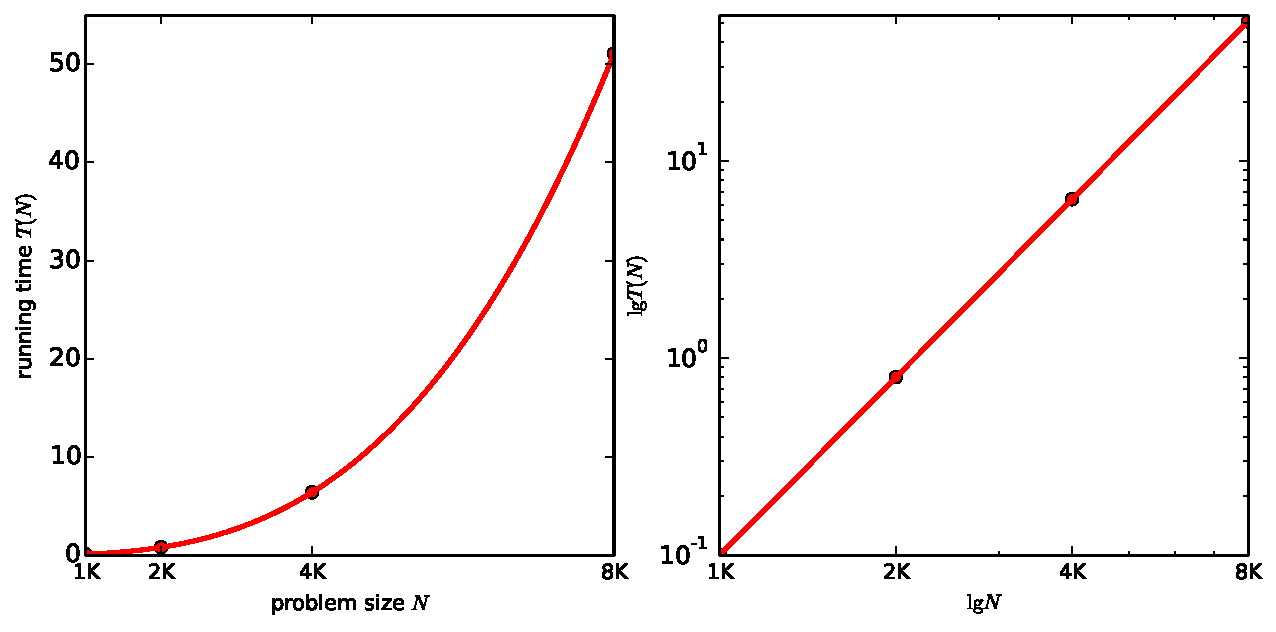
\includegraphics[scale=0.4]{{./figures/threesum}.pdf}}
\end{center}

\pause

From the log-log plot we have $$\lg T(N) = 3\lg N + \lg a,$$ where $a$ is a constant

$$\therefore \text{\ \ \ \ } T(N)=aN^3$$ 
and since $T(8000)=51.1$, we have $$T(N)=9.98\times 10^{-11}N^3$$
\end{frame}

\begin{frame}[fragile]
\pause

We can also derive a mathematical expression for the order of growth $T(N)$ of a program

\pause
\bigskip

The order of growth of a program is determined by: the cost of executing each statement (property of the computer); and the frequency of execution of each statement (property of the program and the input)

\pause
\bigskip

We write $g(N) \sim f(N)$ (called tilde approximation) to represent any function $g(N)$ that, when divided by $f(N)$, approaches 1 as $N$ approaches $\infty$

\pause
\bigskip

Most often, we work with tilde approximations of the form $g(N)\sim af(N)$ where $f(N)=N^b(\log N)^c$ and $a, b$, and $c$ are constants; we refer to $f(N)$ as the order of growth of $g(N)$
\end{frame}

\begin{frame}[fragile]
\pause

Analyzing the order of growth of \lstinline{ThreeSum.count()}
\begin{lstlisting}[language=Java, mathescape]
public static int count(int[] a) {
    int N = a.length;                           $[A]$
    int cnt = 0;
    for (int i = 0; i < N; i++) {               $[B]$ 
        for (int j = i + 1; j < N; j++) {       $[C]$
            for (int k = j + 1; k < N; k++) {   $[D]$
                if (a[i] + a[j] + a[k] == 0) {
                    cnt++;                      $[E]$
                }
            }
        }
    }
    return cnt;
}
\end{lstlisting}

\pause

\begin{center}
\begin{tabular}{cccc}
statement block & time & frequency & total time\\ \hline
$[A]$ & $t_4$ & $1$  & $t_4$ \\
$[B]$ & $t_3$ & $N$  & $t_3N$ \\
$[C]$ & $t_2$ & $N^2/2-N/2$  & $t_2(N^2/2-N/2)$ \\
$[D]$ & $t_1$ & $N^3/6-N^2/2+N/3$  & $t_1(N^3/6-N^2/2+N/3)$ \\
$[E]$ & $t_0$ & $x$ (depends on input) & $t_0x$
\end{tabular} 
\end{center}

\pause

Grand total: $(t_1/6)N^3+(t_2/2-t_1/2)N^2+(t_1/3-t_2/2+t_3)N+t_4+t_0x$

\pause
\smallskip

Tilde approximation: $\sim(t_1/6)N^3$ (assuming $x$ is small)

\pause
\smallskip

Order of growth: $N^3$
\end{frame}

\begin{frame}[fragile]
\pause

For many programs, developing a mathematical model of order of growth reduces to the following steps
\begin{itemize}
\item Develop an input model, including a definition of the problem size
\item Identify the inner loop
\item Define a cost model that includes operations in the inner loop
\item Determine the frequency of execution of those operations for the given input
\end{itemize}

\pause
\bigskip

For \lstinline{ThreeSum}
\begin{itemize}
\item The input model is $N$ numbers
\item The inner loop is the if-statement inside a triply nested \lstinline{for} loop
\item The cost model is the number of array accesses
\item The frequency of array accesses is $N^3/2$
\end{itemize}
\end{frame}

\begin{frame}[fragile]
\pause

Order-of-growth classifications
\begin{center}
\begin{tabular}{cccc}
description & function & code description & example \\ \hline
constant & 1 & statement & add two numbers \\
logarithmic & $\log N$ & divide in half & binary search \\
linear & $N$ & loop & find the maximum \\
linearithmic & $N\log N$ & divide and conquer & merge sort \\
quadratic & $N^2$ & double loop & check all pairs \\
cubic & $N^3$ & triple loop & check all triples \\
exponential & $2^N$ & exhaustive search & check all subsets
\end{tabular} 
\end{center}

\pause
\smallskip

\begin{center}
\visible<3->{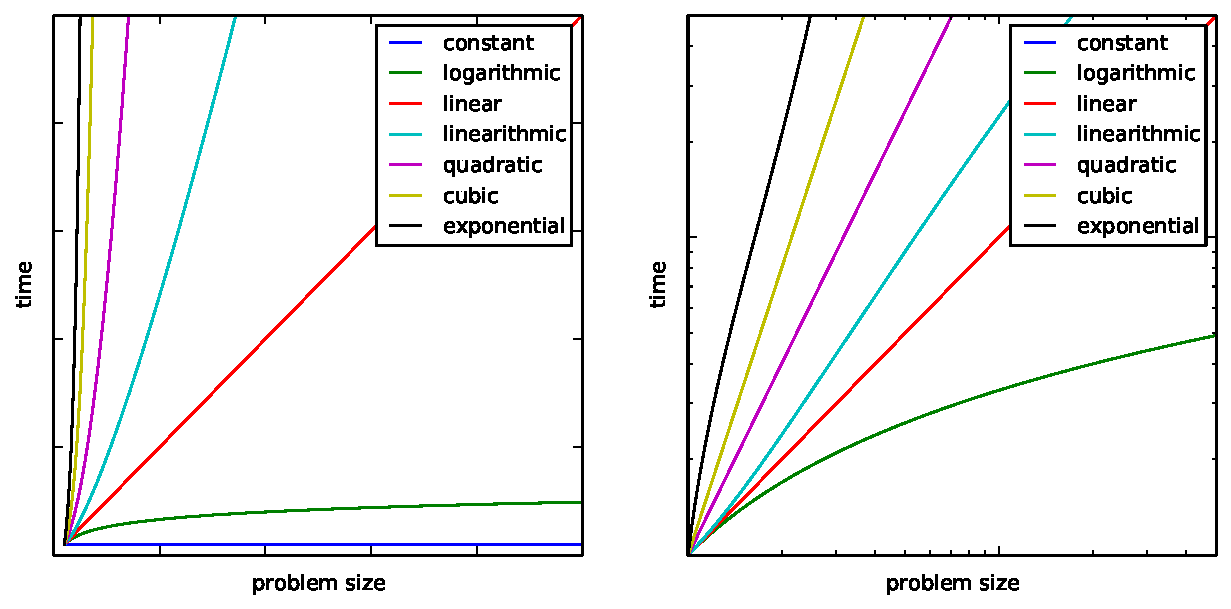
\includegraphics[scale=0.47]{{./figures/order_of_growth}.pdf}}
\end{center}
\end{frame}

\begin{frame}[fragile]
\pause

Search problem: search for a key in a collection of $N$ keys

\pause
\bigskip

Linear search
\begin{lstlisting}[language=Java]
public static int indexOf(int[] a, int key) {
    for (int i = 0; i < a.length; i++) {
        if (a[i] == key) { 
            return i; 
        }
    }
    return -1;
}
\end{lstlisting}

\pause

Order of growth: $N$

\pause
\bigskip

Binary search (successful search for the key 23)
\begin{center}
\visible<5->{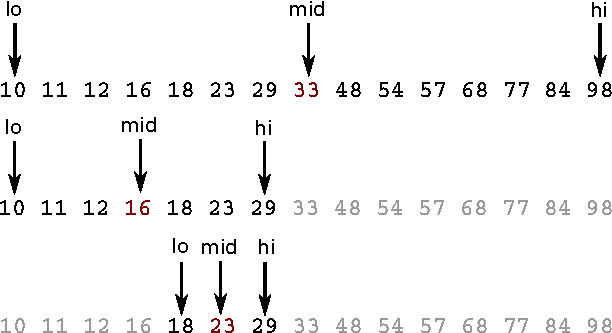
\includegraphics[scale=0.65]{./figures/bs1.pdf}}
\end{center}
\end{frame}

\begin{frame}[fragile]
\pause

Binary search (unsuccessful search for the key 50)
\begin{center}
\visible<2->{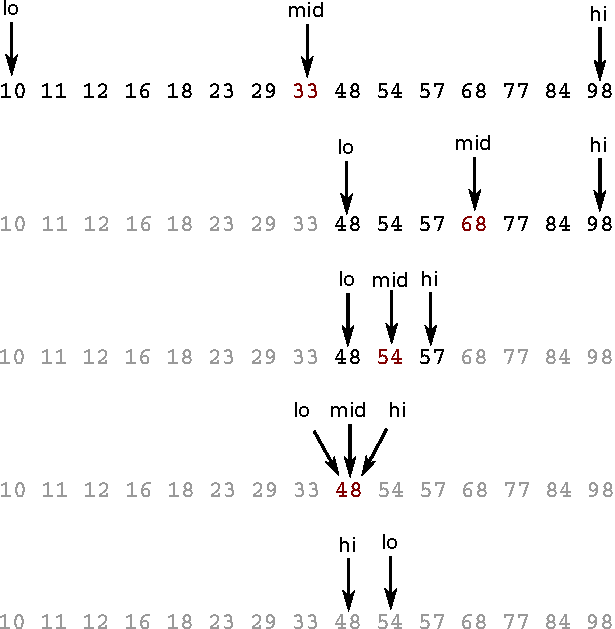
\includegraphics[scale=0.65]{./figures/bs2.pdf}}
\end{center}
\end{frame}

\begin{frame}[fragile]
\pause

Binary search and whitelisting

\begin{lstlisting}[language=Java]
package edu.princeton.cs.algs4;

import java.util.Arrays;

public class BinarySearch {
    public static int indexOf(int[] a, int key) {
        int lo = 0;
        int hi = a.length - 1;
        while (lo <= hi) {
            int mid = lo + (hi - lo) / 2;
            if      (key < a[mid]) { hi = mid - 1; }
            else if (key > a[mid]) { lo = mid + 1; }
            else { return mid; }
        }
        return -1;
    }

    public static void main(String[] args) {
        In in = new In(args[0]);
        int[] whitelist = in.readAllInts();
        Arrays.sort(whitelist);
        while (!StdIn.isEmpty()) {
            int key = StdIn.readInt();
            if (BinarySearch.indexOf(whitelist, key) == -1) {
                StdOut.println(key);
            }
        }
    }
}
\end{lstlisting}
\end{frame}

\begin{frame}[fragile]
\pause

\begin{lstlisting}[language={}]
tinyW.txt tinyT.txt
   84        23
   48        50
   68        10
   10        99
   18        18
   98        23
   12        98
   23        84
   54        11
   57        10
   48        48
   33        77
   16        13
   77        54
   11        98
   29        77
             77
             68
\end{lstlisting}

\pause

\begin{lstlisting}[language={}]
$ java edu.princeton.cs.algs4.BinarySearch tinyW.txt < tinyT.txt
50
99
13
\end{lstlisting}

\pause
\bigskip

Binary search order of growth: $\lg N$ 

\pause
\bigskip

Whitelisting order of growth: $M\lg N$, where $M$ is the number of calls to \lstinline{BinarySearch.indexOf()}, ie, the number of binary searches
\end{frame}

\begin{frame}[fragile]
\pause

Faster solution to the 3-sum problem
\begin{lstlisting}[language=Java]
package edu.princeton.cs.algs4;

import java.util.Arrays;

public class ThreeSumFast {
    public static int count(int[] a) {
        int N = a.length;
        Arrays.sort(a);
        int cnt = 0;
        for (int i = 0; i < N; i++) {
            for (int j = i + 1; j < N; j++) {
                if (BinarySearch.indexOf(a, -a[i] - a[j]) > j) {
                    cnt++;
                }
            }
        }
        return cnt;
    }
    
    public static void main(String[] args) {
        In in = new In(args[0]);
        int[] a = in.readAllInts();
        int cnt = count(a);
        StdOut.println(cnt);
    }
}
\end{lstlisting}

\pause

Order of growth: $N^2\lg N$
\end{frame}

\section{Space Complexity}
\begin{frame}[fragile]
\pause

Memory requirements for primitive types
\begin{center}
\begin{tabular}{cc}
type & bytes \\ \hline
\lstinline$boolean$ & 1 \\
\lstinline$byte$ & 1 \\
\lstinline$char$ & 2 \\
\lstinline$int$ & 4 \\
\lstinline$float$ & 4 \\
\lstinline$long$ & 8 \\
\lstinline$double$ & 8
\end{tabular} 
\end{center}

\pause
\bigskip

To determine the memory usage of an object, we add the amount of memory used by each instance variable to the overhead associated with each object, which is 16 bytes

\pause
\bigskip

A \lstinline{Counter} object uses 32 bytes: 16 bytes of overhead, 8 bytes for its \lstinline{String} instance variable (a reference), 4 bytes for its \lstinline{int} instance variable, and 4 bytes of padding

\pause
\bigskip

A nested non-static (inner) class requires an extra 8 bytes of overhead (for reference to the enclosing instance)
\end{frame}

\begin{frame}[fragile]
\pause

An array of primitive-type values typically requires 24 bytes of header information (16 bytes of object overhead, 4 bytes for the length, and 4 bytes of padding) plus the memory needed to store the values

\pause
\bigskip

For example, an array of $N$ \lstinline{int} values uses $24 + 4N$ bytes 

\pause
\bigskip

An array of objects is an array of references to objects, so we need to add the space for the references to the space required for the objects

\pause
\bigskip

For example, an array of $N$ \lstinline{Date} objects uses 24 bytes (array overhead) plus $8N$ bytes (references) plus 32 bytes for each object, for a grand total of $24+40N$ bytes

\pause
\bigskip

A two-dimensional array is an array of arrays (each array is an object)

\pause
\bigskip

For example, a two-dimensional $M$-by-$N$ array of \lstinline{double} values uses 24 bytes (overhead for array of arrays) plus $8M$ bytes (references to the row arrays) plus $24M$ bytes (overhead from the row arrays) plus $8MN$ bytes (for the $N$ \lstinline{double} values in each of the $M$ rows) for a grand total of $8MN+32M+24\sim 8MN$ bytes

\pause
\bigskip

A \lstinline{String} of length $N$ typically uses 32 bytes (for the \lstinline{String} object) plus $24+2N$ bytes (for the array that contains the characters) for a total of $56+2N$ bytes
\end{frame}
\end{document}
